% !TeX root = Bericht.tex
% !TeX spellcheck = en_US
\section{Setup and procedure}
In this chapter, the execution of the experiments is described. In all following experiments a HeNe laser with a wavelength of $\lambda = 633 \unit{nm}$ is used. In the first part of the experiment a Mach-Zehnder interferometer is constructed. 
Firstly, the laser beam is directed through a polarizer and two mirrors before it is split by a 50/50 beam splitter. Both beams are redirected via a mirror, and pointed again onto a 50/50 beam splitter. Afterwards, the beam passes a mirror, an intensity filter and a collimating lens, before hitting a photodiode, connected to an oscilloscope. All optical elements have to be carefully placed, to have parallel beams exiting the interferometer, leading to interference along the following optical path. Rough alignment is best done by projecting the laser beams onto a far object, like a wall, and adjusting the mirrors position and inclination angles to get the laser spots to align at all distances. Afterwards, fine adjustments can be made by beam walking the laser, whilst using the oscilloscopes minimum and maximum readings and \autoref{eqn:contrast} to maximize the contrast. Optimally, the contrast should be more than 90 \%. 

After this alignment, an elecro-optical modulator (EOM) containing a \ch{LiNbO3} crystal with length \SI{2.45(1)}{cm} and height \SI{1.8(1)}{mm} is placed in one arm of the interferometer and connected to an amplifier and function generator. At the function generator, a frequency of \SI{30}{Hz} and an amplitude of \SI{3}{V}, which is amplified 100 times by the amplifier, is inserted into the EOM. Now, several measurements (for statistical reasons) are done by saving both, signal of the function generator and the recorded intensity from the oscilloscope. After these measurements, a $\lambda/2$ waveplate is placed after the polarizer to rotate the polarization by \ang{90} and traces from function generator and photodiode are saved multiple times. After this, the frequency is raised from $30 \unit{Hz}$ to $100 \unit{Hz}$ and from here in steps of $100 \unit{Hz}$ until \SI{500}{Hz} are reached. For every step, maximum and minimum intensity are recorded. The setup whole setup can be seen in \autoref{ExperimetAufbau_mach_zehnder}. 

\begin{figure}[H]
	\centering
	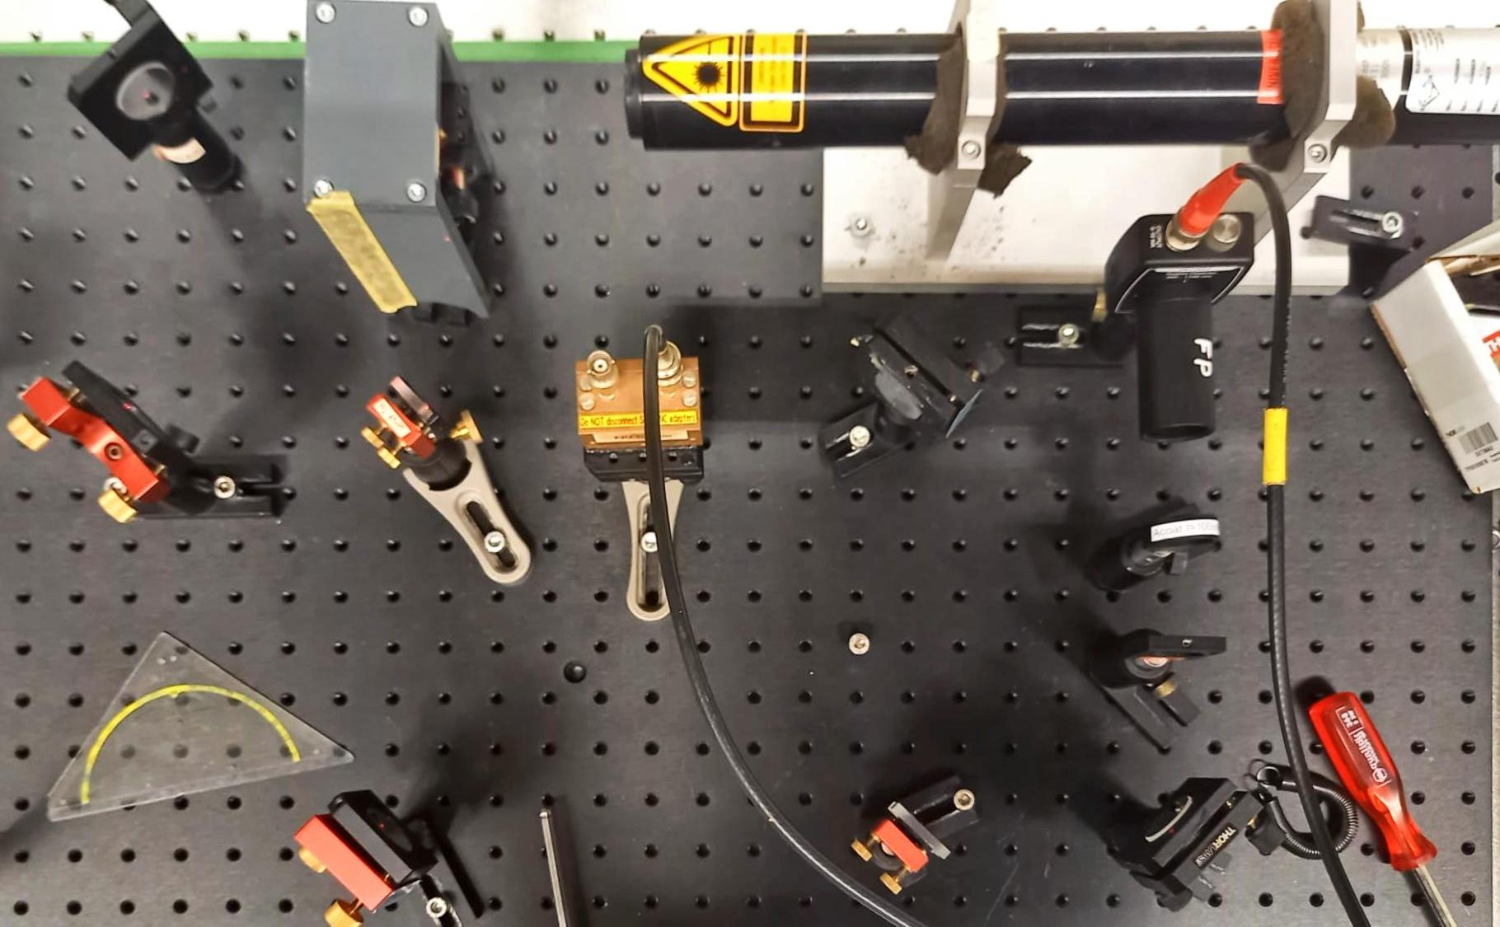
\includegraphics[width=\linewidth]{Aufbau}
	\caption{The setup of the first part of the experiment can be seen. Here light emitted from a \ch{HeNe} laser is polarized and redirected by two mirrors onto a 50-50 beam splitter. This splits the light into two beams, which are directed by two mirrors onto another beam splitter, where, the two beams are brought to interfere. In the top arm an electro-optical modulator (EOM) is placed. In the end, the beam passes an intensity filter, a collimating lens and is recorded by a photodiode.}
	\label{ExperimetAufbau_mach_zehnder}
\end{figure}
The second setup is a much simpler construction and can be seen in \autoref{setup2_eom}. Again, the \ch{HeNe} laser beam is collimated by a lens and redirected by two mirrors. Then, a polarizer and a $\lambda/2$ waveplate are placed, before the EOM. After propagating through the crystal it passes another $\lambda/2$ waveplate and afterwards a polarizer. After a mirror, another collimating lens is placed before the photodiode. As in the interferometer setup, a voltage of \SI{3}{V} and \SI{30}{Hz} is applied, and several measurements are taken. Then, the triangular voltage is switched to a square wave pulse, which lets the EOM to function as an optical switch. The voltage of the driving signal is first approximated from the data already taken and is further fine tuned using the oscilloscopes min/max reading to increase the on/off ratio of the output signal. Now some measurements are taken to determine the on/off ratio. Lastly, the frequency is increased to see the frequency dependent behaviour of the on/off ratio. 

\begin{figure}[H]
	\centering
	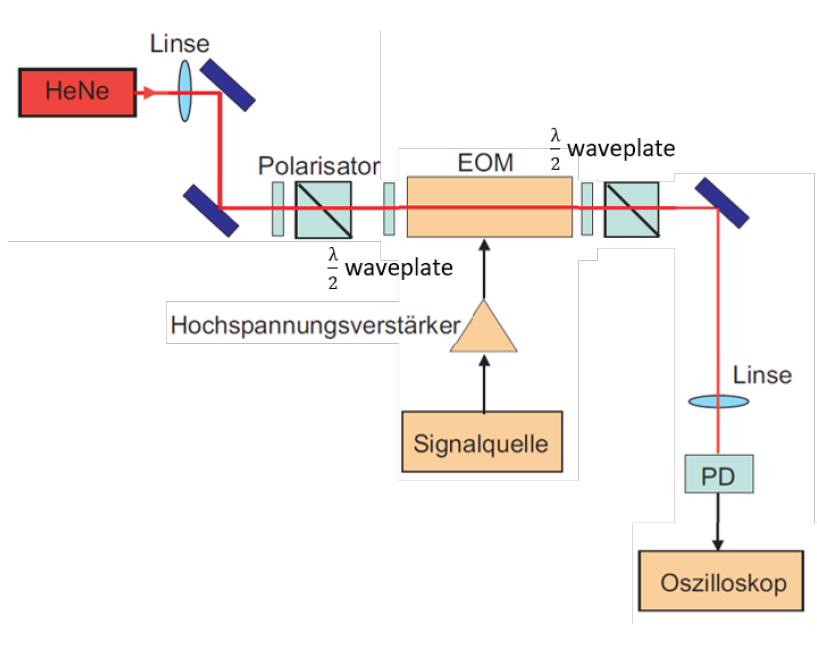
\includegraphics[width=0.6\linewidth]{setup2_eom_richtig.png}
	\caption{The setup of the second part of the experiment is shown. Here light emitted from a \ch{HeNe} laser is polarized and redirected by two mirrors. Waveplates are used to modify the laser's polarization coming into the EOM. Lastly, the beam is collimated by a lens and recorded on an oscilloscope via a photodiode. Figure taken from \autocite{eom}.}
	\label{setup2_eom}
\end{figure}




